\documentclass{beamer}

\usepackage{pgfpages}
\usepackage{caption}
\setbeameroption{show notes on second screen}

\setbeamertemplate{caption}[numbered]
\setbeamerfont{note page}{size=\scriptsize}

\usetheme{Bergen}
\usecolortheme{beetle}

\mode<presentation>

\title{Perbandingan Algoritma \textit{Backtracking} dan Algoritma \textit{Hybrid Genetic} untuk Menyelesaikan Permainan Calcudoku}
\author{Michael Adrian \\ 2013730039 \\ \texttt{michaeladrian39@gmail.com}}
\institute{Jurusan Teknik Informatika \\ Fakultas Teknologi Informasi dan Sains \\ Universitas Katolik Parahyangan}
\date{6 Desember 2016}

\begin{document}

\begin{frame}
\titlepage
\end{frame}

\section{Dasar Teori}

\subsection{Calcudoku}

\begin{frame}
\frametitle{Calcudoku}
\begin{itemize}
\item Salah satu jenis permainan teka-teki aritmatika dan logika
\item Dikenal juga sebagai KenKen, KenDoku, atau Mathdoku
\item Diciptakan pada tahun 2004 oleh Tetsuya Miyamoto, seorang guru matematika dari Jepang
\item Diciptakan untuk melatih kemampuan matematika dan logika dengan cara yang menyenangkan
\end{itemize}
\end{frame}

\note{
Sebagai salah satu jenis permainan teka-teki aritmatika dan \textit{grid}, Calcudoku, atau dikenal juga sebagai KenKen, KenDoku, atau Mathdoku, diciptakan pada tahun 2004 oleh seorang guru matematika dari Jepang yang bernama Tetsuya Miyamoto untuk memenuhi tujuannya untuk melatih kemampuan matematika dan logika siswa-siswinya dengan cara yang menyenangkan. Nama KenKen diambil dari kata bahasa Jepang yang berarti kepandaian. Permainan yang mengasah otak ini dengan cepat menyebar ke seluruh Jepang dan Amerika Serikat, menggantikan permainan teka-teki silang di banyak koran. Permainan ini kemudian menjadi sensasi di seluruh dunia setelah munculnya versi \textit{online} dan \textit{mobile} dari permainan teka-teki ini, khususnya menarik untuk pecinta permainan teka-teki angka seperti Sudoku.
}

\begin{frame}
\frametitle{Aturan Permainan}
\begin{itemize}
\item Pemain diberikan sebuah \textit{grid} dengan ukuran \begin{math}n \times n\end{math}
\item \begin{math}n\end{math} biasanya antara 3 sampai dengan 9
\item \textit{Grid} ini harus diisi dengan angka 1 sampai dengan \begin{math}n\end{math}
\item Dalam setiap baris setiap angka hanya muncul sekali
\item Dalam setiap kolom setiap angka hanya muncul sekali
\item \textit{Grid} dibagi ke dalam \textit{cage}
\item \textit{Cage} adalah sekelompok sel yang dibatasi oleh garis yang lebih tebal daripada garis pembatas antar sel dengan angka tujuan dan operator yang telah ditentukan
\item Angka-angka dalam setiap \textit{cage} harus mencapai angka tujuan jika dihitung menggunakan operator yang telah ditentukan
\item Angka tujuan dan operasi yang telah ditentukan ditulis di sudut kiri atas \textit{cage}
\end{itemize}
\end{frame}

\note{
Seperti dalam Sudoku, dalam teka-teki ini, pemain diberikan sebuah \textit{grid} dengan ukuran \begin{math}n \times n\end{math}, dengan \begin{math}n\end{math} biasanya antara 3 sampai dengan 9. \textit{Grid} ini harus diisi dengan angka 1 sampai dengan \begin{math}n\end{math} sehingga dalam setiap baris setiap angka hanya muncul sekali, dalam setiap kolom setiap angka hanya muncul sekali. Perbedaannya dengan Sudoku adalah, Calcudoku dibagi ke dalam \textit{cage} (sekelompok sel yang dibatasi oleh garis yang lebih tebal daripada garis pembatas antar sel dengan angka tujuan dan operator yang telah ditentukan), dan angka-angka dalam setiap \textit{cage} harus mencapai angka tujuan jika dihitung menggunakan operator yang telah ditentukan. Angka tujuan dan operasi yang telah ditentukan ditulis di sudut kiri atas \textit{cage}.
}

\begin{frame}
\frametitle{Operator-Operator Matematika}
\begin{itemize}
\item Ada 5 kemungkinan operator:
	\begin{itemize}
	\item + (penjumlahan)
	\item - (pengurangan)
	\item \begin{math}\times\end{math} (perkalian)
	\item \begin{math}\div\end{math} (pembagian)
	\item = (sama dengan)
	\end{itemize}
\item Jika operasi matematika yang ditentukan adalah pengurangan atau pembagian, maka ukuruan \textit{cage} harus berukuran dua sel
\end{itemize}
\end{frame}

\note{
Ada lima kemungkinan operator:
\begin{enumerate}
\item +, sebuah operator \begin{math}n\end{math}-ary yang menandakan penjumlahan.
\item -, sebuah operator biner yang menandakan pengurangan.
\item \begin{math}\times\end{math}, sebuah operator  \begin{math}n\end{math}-ary yang menandakan perkalian.
\item \begin{math}\div\end{math} sebuah operator biner yang menandakan pembagian.
\item =, (simbol ini biasanya dihilangkan), sebuah operator uner yang menandakan persamaan.
\end{enumerate}
Jika operasi matematika yang ditentukan adalah pengurangan atau pembagian, maka ukuruan \textit{cage} harus berukuran dua sel. Pada beberapa versi dari teka-teki ini, hanya angka tujuan yang diberikan, dan pemain harus menebak operator dari setiap \textit{cage} untuk menyelesaikan teka-tekinya.
}

\begin{frame}
\frametitle{Contoh Permainan}
\begin{figure}
\centering
\captionsetup{justification=centering}
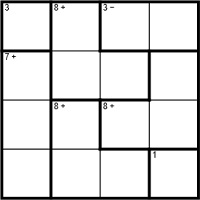
\includegraphics[scale=1]{Gambar/Backtracking1}
\caption[Contoh permainan teka-teki Calcudoku dengan ukuran \textit{grid} 4 x 4 yang belum diselesaikan. ]{Contoh permainan teka-teki dengan ukuran \textit{grid} 4 x 4 yang belum diselesaikan. }
\label{fig:backtracking1}
\end{figure}
\end{frame}

\begin{frame}
\frametitle{Contoh Solusi}
\begin{figure}
\centering
\captionsetup{justification=centering}
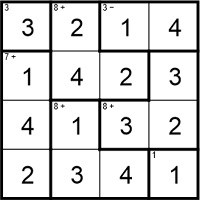
\includegraphics[scale=1]{Gambar/Backtracking2}
\caption[Solusi untuk permainan teka-teki Calcudoku yang diberikan pada Gambar~\ref{fig:backtracking1} ]{Solusi untuk permainan teka-teki Calcudoku yang diberikan pada Gambar~\ref{fig:backtracking1}. }
\label{fig:backtracking2}
\end{figure}
\end{frame}


\begin{frame}
\frametitle{Permasalahan Utama dalam Menyelesaikan Calcudoku}
\begin{itemize}
\item Untuk menyelesaikan sebuah teka-teki Calcudoku, pemain harus pertama-tama memahami dua permasalahan utama dari teka-teki ini, yaitu:
	\begin{itemize}
	\item Angka-angka mana yang harus dimasukkan ke dalam sebuah \textit{cage}
	\item Dalam urutan apa angka-angka tersebut harus dimasukkan ke dalam sebuah \textit{cage}
	\end{itemize}
\item Cara yang paling mudah untuk menyelesaikan teka-teki ini adalah dengan mengeliminasi angka-angka yang sudah digunakan dan mencoba satu per satu angka yang mungkin (\textit{trial and error}). 
\end{itemize}
\end{frame}

\note{
Untuk menyelesaikan sebuah teka-teki Calcudoku, pemain harus pertama-tama memahami dua permasalahan utama dari teka-teki ini, yaitu:
\begin{enumerate}
\item Angka-angka mana yang harus dimasukkan ke dalam sebuah \textit{cage}
\item Dalam urutan apa angka-angka tersebut harus dimasukkan ke dalam sebuah \textit{cage}
\end{enumerate}

Seperti kebanyakan permainan teka-teki angka, cara yang paling mudah untuk menyelesaikan teka-teki ini adalah dengan mengeliminasi angka-angka yang sudah digunakan dan mencoba satu per satu angka yang mungkin (\textit{trial and error}). 
}

\begin{frame}
\frametitle{Tahapan Pengisian Calcudoku}
\begin{itemize}
\item Dalam pengisian teka-teki ini ada dua tahapan, yaitu:
	\begin{itemize}
	\item Mencari \textit{cage} yang hanya berukuran 1 sel
	\item Mencari mencari \textit{cage} yang hanya mempunyai satu kemungkinan kombinasi angka
	\end{itemize}
\end{itemize}
\end{frame}

\note{
Dalam pengisian teka-teki ini ada dua tahapan, yaitu:
\begin{enumerate} 
\item Mencari \textit{cage} yang hanya berukuran 1 sel, karena \textit{cage} ini tidak menghasilkan pertanyaan angka apa dan urutan apa. Tahap ini adalah tahap yang paling jelas. Contoh, pada Gambar~\ref{fig:backtracking1}, \textit{cage} pada sudut kiri atas dan \textit{cage} pada sudut kanan bawah hanya berukuran 1 sel, dan dapat langsung diisi dengan angka tujuannya.
\item Mencari mencari \textit{cage} yang hanya mempunyai satu kemungkinan kombinasi angka, sehingga masalah angka-angka apa yang harus diisi dalam \textit{cage} tersebut terjawab. Contoh, \textit{cage} pada sudut kanan atas mempunyai aturan "3-", artinya angka tujuannya adalah 3 dengan menggunakan operasi pengurangan. Satu-satunya pasangan angka dari himpunan \{1,2,3,4\} yang akan menghasilkan angka 3 saat satu angka dikurangkan dari angka yang lainnya adalah \{1,4\}. Namun masalahnya adalah urutan angka-angka yang harus dimasukkan. Dalam kasus ini, untungnya, sel pada sudut kanan bawah sudah diisi dengan angka 1, maka angka 1 tidak bisa digunakan lagi pada kolom yang paling kanan. Jadi, dengan menggunakan cara eliminasi, sel pada sudut kanan atas harus diisi dengan angka 4 dan sel di sebelah kirinya, yaitu sel pada baris yang paling atas dan kolom ketiga dari kiri, harus diisi dengan angka 1. Hal ini memberikan solusi untuk sel pada baris yang paling atas dan kolom kedua dari kiri, yaitu angka 2, karena angka 2 adalah angka yang belum pernah dipakai dalam baris tersebut. Proses ini berlanjut sampai semua sel dalam \textit{grid} terisi dan menghasilkan solusi pada Gambar~\ref{fig:backtracking2}.
\end{enumerate}
}

\begin{frame}
\frametitle{Tahapan Pengisian Calcudoku}
\begin{itemize}
\item Seiring dengan meningkatnya tingkat kesulitan, langkah berikutnya tidak akan langsung muncul dengan jelas
\item Kadang-kadang, pemain mencapai titik dimana langkah berikutnya tidak pasti
\item Pemain harus menebak langkah-langkah berikutnya dan melihat apakah langkah ini akan menghasilkan solusinya. Jika tidak, pemain harus mundur kembali ke titik ketidakpastian tersebut.
\end{itemize}
\end{frame}

\note{
Seiring dengan meningkatnya tingkat kesulitan, langkah berikutnya tidak akan langsung muncul dengan jelas. Kadang-kadang, pemain mencapai titik dimana langkah berikutnya tidak pasti. Pemain harus menebak langkah-langkah berikutnya dan melihat apakah langkah ini akan menghasilkan solusinya. Jika tidak, pemain harus mundur kembali ke titik ketidakpastian tersebut.
}

\begin{frame}
\frametitle{Mendefinisikan Permasalahan Calcudoku}
\begin{itemize}
\item Sebuah teka-teki Calcudoku dengan ukuran \begin{math}n \times n\end{math}, dengan \begin{math}n\end{math} melambangkan jumlah sel dalam satu baris atau kolom, mempunyai \begin{math}n^2\end{math} sel
\item Sel yang terletak dalam baris \begin{math}b\end{math} dan kolom \begin{math}k\end{math} diberi label \begin{math}C_{b,k} = bn + k\end{math}
\item Nilai dari sel tersebut adalah \begin{math}V(C_{b,k}) \in \{1, 2, ..., n\}\end{math}.
\item Sebuah \textit{cage}, yang diberi label \begin{math}A_i\end{math} adalah sebuah himpunan dari sel, yaitu \begin{math}A_i = \{C_{b,k}\}\end{math}
\item Setiap \textit{cage} terhubung dengan satu operator aritmatika \begin{math}O_i \in \{+, -, \times, \div\}, =\end{math} dan satu angka tujuan \begin{math}H_i \in N\end{math}
\end{itemize}
\end{frame}

\note{
Sebuah teka-teki Calcudoku dengan ukuran \begin{math}n \times n\end{math}, dengan \begin{math}n\end{math} melambangkan jumlah sel dalam satu baris atau kolom, mempunyai \begin{math}n^2\end{math} sel. Sel yang terletak dalam baris \begin{math}b\end{math} dan kolom \begin{math}k\end{math} diberi label \begin{math}C_{b,k} = bn + k\end{math} dan nilai dari sel tersebut adalah \begin{math}V(C_{b,k}) \in \{1, 2, ..., n\}\end{math}. Sebuah \textit{cage}, yang diberi label \begin{math}A_i\end{math} adalah sebuah himpunan dari sel, yaitu \begin{math}A_i = \{C_{b,k}\}\end{math}. Setiap \textit{cage} terhubung dengan satu operator aritmatika \begin{math}O_i \in \{+, -, \times, \div\}\end{math} dan satu angka tujuan \begin{math}H_i \in N\end{math}.
}

\begin{frame}
\frametitle{Mendefinisikan Permasalahan Calcudoku}
\begin{itemize}
\item 3 aturan dalam mendefinisikan masalah dalam Calcudoku adalah sebagai berikut
	\begin{itemize}
	\item \begin{math}|A_i| = 1 \rightarrow O_i = \phi\end{math}, artinya setiap \textit{cage} yang jumlah selnya 1 dengan operasi matematika yang terkait dengan \textit{cage} tersebut bersifat homeomorfik (setara).
	\item \begin{math}O_i \in {-, \div} \rightarrow |A_i| = 2\end{math}, artinya jika operasi yang digunakan dalam sebuah \textit{cage} adalah pengurangan atau pembagian, maka jumlah sel dalam \textit{cage} tersebut harus 2.
	\item \begin{math}\forall C_{b,k} \rightarrow C_{b,k} \in \exists! A_i\end{math}, artinya setiap sel hanya boleh menjadi anggota dari satu dan hanya satu \textit{cage}.
	\end{itemize}
\end{itemize}
\end{frame}

\note{
Menurut Johanna, Lukas, dan Saputra, tiga aturan dalam mendefinisikan masalah dalam Calcudoku adalah sebagai berikut:
\begin{enumerate}
\item \begin{math}|A_i| = 1 \rightarrow O_i = \phi\end{math}, artinya setiap \textit{cage} yang jumlah selnya 1 dengan operasi matematika yang terkait dengan \textit{cage} tersebut bersifat homeomorfik (setara)
\item \begin{math}O_i \in {-, \div} \rightarrow |A_i| = 2\end{math}, artinya jika operasi yang digunakan dalam sebuah \textit{cage} adalah pengurangan atau pembagian, maka jumlah sel dalam \textit{cage} tersebut harus 2
\item \begin{math}\forall C_{b,k} \rightarrow C_{b,k} \in \exists! A_i\end{math}, artinya setiap sel hanya boleh menjadi anggota dari satu dan hanya satu \textit{cage}
\end{enumerate}
}

\begin{frame}
\frametitle{Mendefinisikan Permasalahan Calcudoku}
\begin{itemize}
\item Tujuan dari teka-teki ini adalah untuk mencari nilai \begin{math}V(C_{b,k})\end{math} dan memenuhi persyaratan berikut
	\begin{itemize}
	\item \begin{math}|A_i| = 1 \land C_{b,k} \in A_i \rightarrow V(C_{b,k}) = H_i\end{math}, artinya jika sel adalah bagian dari sebuah \textit{cage} yang jumlah selnya 1, maka nilai dari sel tersebut adalah angka tujuan dari \textit{cage} tersebut
	\item \begin{math}O_i \in \{-\} \land A_i = \{C_{a,b}, C_{p,q}\} \rightarrow |V(C_{a,b}) - V(C_{p,q})| = H_i\end{math}, artinya nilai absolut dari hasil pengurangan nilai kedua sel di dalam \textit{cage} tersebut adalah angka tujuan dari \textit{cage} tersebut
	\item \begin{math}O_i \in \{\div\} \land A_i = \{C_{a,b}, C_{p,q}\} \rightarrow V(C_a,_b) / V(C_{p,q}) = H_i\end{math}, artinya nilai dari hasil pembagian nilai kedua sel di dalam \textit{cage} tersebut adalah angka tujuan dari \textit{cage} tersebut
	\item \begin{math}O_i \in \{+\} \rightarrow \sum_{C_{b,k} \in A_i} V(C_{b,k}) = H_i\end{math}, artinya nilai dari hasil penjumlahan dari nilai semua sel di dalam \textit{cage} tersebut adalah angka tujuan dari \textit{cage} tersebut
	\item \begin{math}O_i \in \{\times\} \rightarrow \prod_{C_{b,k} \in A_i} V(C_{b,k}) = H_i\end{math}, artinya nilai dari hasil perkalian dari nilai semua sel di dalam \textit{cage} tersebut adalah angka tujuan dari \textit{cage} tersebut
	\end{itemize}
\end{itemize}
\end{frame}

\note{
Menurut Johanna, Lukas, dan Saputra, tujuan dari teka-teki ini adalah untuk mencari nilai \begin{math}V(C_{b,k})\end{math} dan memenuhi persyaratan berikut:
\begin{enumerate}
\item \begin{math}|A_i| = 1 \land C_{b,k} \in A_i \rightarrow V(C_{b,k}) = H_i\end{math}, artinya jika sel adalah bagian dari sebuah \textit{cage} yang jumlah selnya 1, maka nilai dari sel tersebut adalah angka tujuan dari \textit{cage} tersebut.
\item \begin{math}O_i \in \{-\} \land A_i = \{C_{a,b}, C_{p,q}\} \rightarrow |V(C_{a,b}) - V(C_{p,q})| = H_i\end{math}, artinya jika sebuah \textit{cage} yang operasi matematikanya adalah pengurangan, maka nilai absolut dari hasil pengurangan nilai kedua sel di dalam \textit{cage} tersebut adalah angka tujuan dari \textit{cage} tersebut.
\item \begin{math}O_i \in \{\div\} \land A_i = \{C_{a,b}, C_{p,q}\} \rightarrow V(C_a,_b) / V(C_{p,q}) = H_i\end{math}, artinya jika sebuah \textit{cage} yang operasi matematikanya adalah pembagian, maka nilai dari hasil pembagian nilai kedua sel di dalam \textit{cage} tersebut adalah angka tujuan dari \textit{cage} tersebut.
\item \begin{math}O_i \in \{+\} \rightarrow \sum_{C_{b,k} \in A_i} V(C_{b,k}) = H_i\end{math}, artinya jika sebuah \textit{cage} yang operasi matematikanya adalah penjumlahan, maka nilai dari hasil penjumlahan dari nilai semua sel di dalam \textit{cage} tersebut adalah angka tujuan dari \textit{cage} tersebut.
\item \begin{math}O_i \in \{\times\} \rightarrow \prod_{C_{b,k} \in A_i} V(C_{b,k}) = H_i\end{math}, artinya jika sebuah \textit{cage} yang operasi matematikanya adalah perkalian, maka nilai dari hasil perkalian dari nilai semua sel di dalam \textit{cage} tersebut adalah angka tujuan dari \textit{cage} tersebut.
\end{enumerate}
}

\subsection{Algoritma \protect\textit{Backtracking}}

\begin{frame}
\frametitle{Algoritma \protect\textit{Backtracking}}
\begin{itemize}
\item Sebuah algoritma umum yang mencari solusi dengan mencoba salah satu dari beberapa pilihan, jika pilihan yang dipilih ternyata salah, komputasi dimulai lagi pada titik pilihan dan mencoba pilihan lainnya
\item Untuk bisa melacak kembali langkah-langkah yang telah dipilih, maka algoritma harus secara eksplisit menyimpan jejak dari setiap langkah yang sudah pernah dipilih, atau menggunakan rekursi (\textit{recursion})
\item Rekursi dipilih karena jauh lebih mudah daripada harus menyimpan jejak setiap langkah yang pernah dipilih
\item Hal ini menyebabkan algoritma ini biasanya berbasis DFS (\textit{Depth First Search})
\end{itemize}
\end{frame}

\note{
Algoritma \textit{backtracking} adalah sebuah algoritma umum yang mencari solusi dengan mencoba salah satu dari beberapa pilihan, jika pilihan yang dipilih ternyata salah, komputasi dimulai lagi pada titik pilihan dan mencoba pilihan lainnya. Untuk bisa melacak kembali langkah-langkah yang telah dipilih, maka algoritma harus secara eksplisit menyimpan jejak dari setiap langkah yang sudah pernah dipilih, atau menggunakan rekursi (\textit{recursion}). Rekursi dipilih karena jauh lebih mudah daripada harus menyimpan jejak setiap langkah yang pernah dipilih. Hal ini menyebabkan algoritma ini biasanya berbasis DFS (\textit{Depth First Search}).
}

\begin{frame}
\frametitle{Algoritma \protect\textit{Backtracking}}
\begin{itemize}
\item Pertama kali diperkenalkan pada tahun 1950 oleh D.H. Lehmer sebagai perbaikan algoritma \textit{brute force}
\item Algoritma ini terbukti efektif untuk menyelesaikan banyak permainan logika karena algoritma itu terutama berguna untuk menyelesaikan masalah-masalah \textit{constraint satisfaction}, di mana sekumpulan objek harus memenuhi sejumlah batasan
\end{itemize}
\end{frame}

\note{
Algoritma \textit{backtracking} pertama kali diperkenalkan pada tahun 1950 oleh D.H. Lehmer sebagai perbaikan algoritma \textit{brute force}. Algoritma ini lalu dikembangkan lebih lanjut oleh R.J. Walker, S.W. Golomb, dan L.D. Baumert. Algoritma ini terbukti efektif untuk menyelesaikan banyak permainan logika (misalnya \textit{tic tac toe}, \textit{maze}, catur, dan lain-lain) karena algoritma itu terutama berguna untuk menyelesaikan masalah-masalah \textit{constraint satisfaction}, di mana sekumpulan objek harus memenuhi sejumlah batasan.
}

\begin{frame}
\frametitle{Sifat-Sifat Umum Algoritma \protect\textit{Backtracking}}
\begin{itemize}
\item Implementasi algoritma \textit{backtracking} memiliki beberapa sifat umum, yaitu:
	\begin{itemize}
		\item Ruang solusi (\textit{solution space})
		\item Fungsi pembangkit (\textit{generating function})
		\item Fungsi pembatas (\textit{generating function})
	\end{itemize}
\end{itemize}
\end{frame}

\note{

}

\begin{frame}
\frametitle{Ruang Solusi}
\begin{itemize}
\item Solusi untuk masalah ini dinyatakan sebagai sebuah vektor \begin{math}X\end{math} dengan \textit{\begin{math}n\end{math}-tuple}:
\begin{displaymath}
X = (x_1, x_2, ..., x_n), x_i \in S_i
\end{displaymath}
di mana adalah mungkin bahwa:
\begin{displaymath}
S_1 = S_2 = ... = S_n
\end{displaymath}
\item \begin{math}n\end{math} adalah jumlah sel dalam satu baris atau kolom
\item \begin{math}X\end{math} adalah sebuah \textit{tuple} yang berukuran \begin{math}n^2\end{math}, yang mereprentasikan isi dari setiap sel dalam \textit{grid}, dimulai pada sel pada sudut kiri atas, lalu bergerak ke sel di sebelah kanannya dalam baris yang sama, jika sudah mencapai sel yang paling kanan maka bergerak ke sel yang paling kiri pada baris dibawahnya, hingga berakhir di sel pada sudut kanan bawah
\item \begin{math}S_i\end{math} adalah sebuah himpunan yang berisi angka-angka dari 1 sampai \begin{math}n\end{math}
\end{itemize}
\end{frame}

\note{
\textit{Solution space}
\\ Solusi untuk masalah ini dinyatakan sebagai sebuah vektor \begin{math}X\end{math} dengan \textit{\begin{math}n\end{math}-tuple}:
\begin{displaymath}
X = (x_1, x_2, ..., x_n), x_i \in S_i
\end{displaymath}
di mana adalah mungkin bahwa:
\begin{displaymath}
S_1 = S_2 = ... = S_n
\end{displaymath} 
\begin{math}n\end{math} adalah jumlah sel dalam satu baris atau kolom. \begin{math}X\end{math} adalah sebuah \textit{tuple} yang berukuran \begin{math}n^2\end{math}, yang mereprentasikan isi dari setiap sel dalam \textit{grid}, dimulai pada sel pada sudut kiri atas, lalu bergerak ke sel di sebelah kanannya dalam baris yang sama, jika sudah mencapai sel yang paling kanan maka bergerak ke sel yang paling kiri pada baris dibawahnya, hingga berakhir di sel pada sudut kanan bawah. \begin{math}S_i\end{math} adalah sebuah himpunan yang berisi angka-angka dari 1 sampai \begin{math}n\end{math}.
}

\begin{frame}
\frametitle{Fungsi Pembangkit}
\begin{itemize}
\item Fungsi pembangkit \begin{math}X_k\end{math} dinyatakan sebagai:
\begin{displaymath}
T(k)
\end{displaymath}
di mana \begin{math}T(k)\end{math} membangkitkan nilai \begin{math}X_k\end{math}, dari 1 sampai \begin{math}n\end{math}, yang merupakan komponen dari vektor solusi
\end{itemize}
\end{frame}

\note{
Fungsi pembangkit \begin{math}X_k\end{math}
\\ Fungsi pembangkit \begin{math}X_k\end{math} dinyatakan sebagai:
\begin{displaymath}
T(k)
\end{displaymath}
di mana \begin{math}T(k)\end{math} membangkitkan nilai \begin{math}X_k\end{math}, dari 1 sampai \begin{math}n\end{math}, yang merupakan komponen dari vektor solusi.
}

\begin{frame}
\frametitle{Fungsi Pembatas}
\begin{itemize}
\item Fungsi pembatas dinyatakan sebagai:
\begin{displaymath}
B(x_1, x_2, ..., x_k)
\end{displaymath}
di mana B bernilai \textit{true} jika \begin{math}(x_1, x_2, ..., x_k)\end{math} mengarah ke solusi. Jika B bernilai \textit{true}, maka nilai \begin{math}x_k+1\end{math} akan terus dibangkitkan, dan jika B bernilai \textit{false}, maka \begin{math}(x_1, x_2, ..., x_k)\end{math} akan dibuang
\end{itemize}
\end{frame}

\note{
Fungsi pembangkit \begin{math}X_k\end{math}
Fungsi pembatas
\\ Fungsi pembatas dinyatakan sebagai:
\begin{displaymath}
B(x_1, x_2, ..., x_k)
\end{displaymath}
di mana B bernilai \textit{true} jika \begin{math}(x_1, x_2, ..., x_k)\end{math} mengarah ke solusi. Jika B bernilai \textit{true}, maka nilai \begin{math}x_k+1\end{math} akan terus dibangkitkan, dan jika B bernilai \textit{false}, maka \begin{math}(x_1, x_2, ..., x_k)\end{math} akan dibuang.
}

\begin{frame}
\frametitle{Ruang Solusi}
\begin{itemize}
\item Disusun dalam sebuah struktur berbentuk pohon (\textit{tree})
\item Setiap simpul (\textit{node}) merepresentasikan keadaan masalah
\item Setiap sisi (\textit{edge}) diberi label \begin{math}x_i\end{math}
\item Jalur dari akar (\textit{root}) ke daun (\textit{leaf}) merepresentasikan sebuah jawaban yang mungkin
\item Semua jalur yang dikumpulkan bersama-sama membentuk ruang solusi
\item Struktur pohon ini disebut sebagai \textit{state space tree}
\end{itemize}
\end{frame}

\note{
Ruang solusi untuk algoritma \textit{backtracking} disusun dalam sebuah struktur berbentuk pohon (\textit{tree}), di mana setiap simpul (\textit{node}) merepresentasikan keadaan masalah dan sisi (\textit{edge}) diberi label \begin{math}x_i\end{math}. Jalur dari akar (\textit{root}) ke daun (\textit{leaf}) merepresentasikan sebuah jawaban yang mungkin, dan semua jalur yang dikumpulkan bersama-sama membentuk ruang solusi. Struktur pohon ini disebut sebagai \textit{state space tree}. Gambar~\ref{fig:backtracking3} menggambarkan contoh sebuah \textit{state space tree}.
}

\begin{frame}
\frametitle{Ruang Solusi}
\begin{figure}
\centering
\captionsetup{justification=centering}
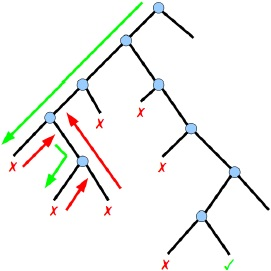
\includegraphics[scale=1]{Gambar/Backtracking3}
\caption[Ilustrasi \textit{State space tree} yang digunakan dalam algoritma  \textit{backtracking}]{Ilustrasi \textit{State space tree} yang digunakan dalam algoritma \textit{backtracking}}
\label{fig:backtracking3}
\end{figure}
\end{frame}

\begin{frame}
\frametitle{Langkah-Langkah Penggunaan \protect\textit{State Space Tree}}
\begin{itemize}
\item Langkah-langkah dalam menggunakan \textit{state space tree} untuk mencari solusi adalah:
\begin{itemize}
	\item Solusi dicari dengan membangun jalur dari akar ke daun menggunakan algoritma DFS
	\item Simpul yang terbentuk disebut sebagai simpul hidup (\textit{live nodes})
	\item Simpul yang sedang diperluas disebut sebagai \textit{expand nodes} atau \textit{E-nodes}
	\item Setiap kali sebuah \textit{E-node} sedang diperluas, jalur yang dikembangkannya menjadi lebih panjang
	\item Jika jalur yang sedang dikembangkan tidak mengarah ke solusi, maka \textit{E-node} dimatikan dan menjadi simpul mati (\textit{dead node})
	\end{itemize}
\end{itemize}
\end{frame}

\note{
Langkah-langkah dalam menggunakan \textit{state space tree} untuk mencari solusi adalah ~\cite{fahda:16:backtracking}:
\begin{itemize}
\item Solusi dicari dengan membangun jalur dari akar ke daun menggunakan algoritma DFS.
\item Simpul yang terbentuk disebut sebagai simpul hidup (\textit{live nodes}).
\item Simpul yang sedang diperluas disebut sebagai \textit{expand nodes} atau \textit{E-nodes}.
\item Setiap kali sebuah \textit{E-node} sedang diperluas, jalur yang dikembangkannya menjadi lebih panjang.
\item Jika jalur yang sedang dikembangkan tidak mengarah ke solusi, maka \textit{E-node} dimatikan dan menjadi simpul mati (\textit{dead node}).
\end{itemize}
}

\begin{frame}
\frametitle{Langkah-Langkah Penggunaan \protect\textit{State Space Tree}}
\begin{itemize}
\item Lanjutan dari slide sebelumnya:
	\begin{itemize}
	\item Fungsi yang digunakan untuk mematikan \textit{E-node} adalah implementasi dari fungsi pembatas
	\item Simpul mati tidak akan diperluas
	\item Jika jalur yang sedang dibangun berakhir dengan simpul mati, proses akan mundur ke simpul sebelumnya
	\item Simpul sebelumnya terus membangkitkan simpul anak (\textit{child node}) lainnya, yang kemudian menjadi \textit{E-node} baru
	\item Pencarian selesai jika simpul tujuan tercapai
	\end{itemize}
\end{itemize}
\end{frame}

\note{
Langkah-langkah dalam menggunakan \textit{state space tree} untuk mencari solusi adalah ~\cite{fahda:16:backtracking}:
\begin{itemize}
\item Fungsi yang digunakan untuk mematikan \textit{E-node} adalah implementasi dari fungsi pembatas.
\item Simpul mati tidak akan diperluas.
\item Jika jalur yang sedang dibangun berakhir dengan simpul mati, proses akan mundur ke simpul sebelumnya.
\item Simpul sebelumnya terus membangkitkan simpul anak (\textit{child node}) lainnya, yang kemudian menjadi \textit{E-node} baru.
\item Pencarian selesai jika simpul tujuan tercapai.
\end{itemize}
}

\begin{frame}
\frametitle{Kompleksitas Waktu}
\begin{itemize}
\item Setiap simpul di dalam \textit{state space tree} terkait dengan panggilan rekursif
\item Jika jumlah simpul di dalam pohon \begin{math}2n\end{math} atau \begin{math}n!\end{math}, maka pada kasus terburuk untuk algoritma \textit{backtracking} ini memiliki kompleksitas waktu \begin{math}O(p(n)2n)\end{math} atau \begin{math}O(q(n)n!)\end{math}, dengan \begin{math}p(n)\end{math} dan \begin{math}q(n)\end{math} sebagai polinomial dengan \begin{math}n\end{math}-derajat menyatakan waktu komputasi untuk setiap simpul
\end{itemize}
\end{frame}

\note{
Setiap simpul di dalam \textit{state space tree} terkait dengan panggilan rekursif. Jika jumlah simpul di dalam pohon \begin{math}2n\end{math} atau \begin{math}n!\end{math}, maka pada kasus terburuk untuk algoritma \textit{backtracking} ini memiliki kompleksitas waktu \begin{math}O(p(n)2n)\end{math} atau \begin{math}O(q(n)n!)\end{math}, dengan \begin{math}p(n)\end{math} dan \begin{math}q(n)\end{math} sebagai polinomial dengan \begin{math}n\end{math}-derajat menyatakan waktu komputasi untuk setiap simpul.
}

\begin{frame}
\frametitle{Ruang Solusi}
\begin{itemize}
\item Ruang solusi untuk sebuah permainan teka-teki Calcudoku dengan \textit{grid} yang berukuran \begin{math}n \times n\end{math} adalah \begin{math}X = (x_1,x_2,...,x_m), x_i \in \{1,2,...,n\}\end{math}, dengan \begin{math}m = n^2\end{math}
\item Fungsi pembangkit membangkitkan sebuah integer secara berurutan dari 1 sampai \begin{math}n\end{math} sebagai \begin{math}x_k\end{math}
\item Fungsi pembatas menggabungkan tiga fungsi pemeriksa pembatas (\textit{constraint checking}), yaitu:
	\begin{itemize}
	\item Fungsi pemeriksa kolom (\textit{column checking})
	\item Fungsi pemeriksa baris (\textit{row checking})
	\item Fungsi pemeriksa \textit{grid} (\textit{grid checking})
	\end{itemize}
\end{itemize}
\end{frame}

\note{
Ruang solusi untuk sebuah permainan teka-teki Calcudoku dengan \textit{grid} yang berukuran \begin{math}n \times n\end{math} adalah \begin{math}X = (x_1,x_2,...,x_m), x_i \in \{1,2,...,n\}\end{math}, dengan \begin{math}m = n^2\end{math}. Fungsi pembangkit membangkitkan sebuah integer secara berurutan dari 1 sampai \begin{math}n\end{math} sebagai \begin{math}x_k\end{math}. Fungsi pembatas menggabungkan tiga fungsi pemeriksa pembatas (\textit{constraint checking}), yaitu fungsi pemeriksa kolom (\textit{column checking}), fungsi pemeriksa baris (\textit{row checking}), dan fungsi pemeriksa \textit{grid} (\textit{grid checking}).
}

\begin{frame}
\frametitle{Fungsi Pembatas}
\begin{itemize}
\item Fungsi pemeriksa kolom menghasilkan nilai \textit{true} jika \begin{math}x_k\end{math} belum ada di dalam kolom dan menghasilkan nilai \textit{false} jika sebaliknya
\item Fungsi pemeriksa baris menghasilkan nilai \textit{true} jika \begin{math}x_k\end{math} belum ada di dalam baris dan menghasilkan nilai \textit{false} jika sebaliknya
\item Fungsi pemeriksa \textit{grid} memeriksa operator pada \textit{grid} dan memeriksa berdasarkan operator yang telah ditentukan
\end{itemize}
\end{frame}

\note{
Fungsi pemeriksa kolom menghasilkan nilai \textit{true} jika \begin{math}x_k\end{math} belum ada di dalam kolom dan menghasilkan nilai \textit{false} jika \begin{math}x_k\end{math} sudah ada di dalam kolom.

Fungsi pemeriksa baris menghasilkan nilai \textit{true} jika \begin{math}x_k\end{math} belum ada di dalam baris dan menghasilkan nilai \textit{false} jika \begin{math}x_k\end{math} sudah ada di dalam baris.

Fungsi pemeriksa \textit{grid} memeriksa operator pada \textit{grid} dan memeriksa berdasarkan operator yang telah ditentukan.
}

\begin{frame}
\frametitle{Operator-Operator untuk Fungsi Pemeriksa \protect\textit{Grid}}
\begin{itemize}
\item Ada 5 operator yang digunakan dalam fungsi ini, yaitu:
	\begin{itemize}
	\item Operator penjumlahan (+), fungsi menghasilkan nilai \textit{true} jika hasil penjumlahan semua nilai yang ada pada \textit{grid} ditambah dengan \begin{math}x_k\end{math} kurang dari atau sama dengan nilai tujuan, dan menghasilkan nilai \textit{false} jika sebaliknya
	\item Operator pengurangan (-), fungsi menghasilkan nilai \textit{true} jika kedua sel dalam \textit{grid} kosong, atau jika ada satu sel yang kosong dan hasil dari \begin{math}x_k\end{math} dikurangi dengan nilai dari sel yang lainnya atau hasil dari nilai dari sel yang lainnya dikurangi dengan \begin{math}x_k\end{math} menghasilkan nilai tujuan, dan menghasilkan nilai \textit{false} jika sebaliknya
	\end{itemize}
\end{itemize}
\end{frame}

\note{
Ada 5 operator yang digunakan dalam fungsi ini, yaitu:
\begin{itemize}
\item Operator penjumlahan (+), fungsi menghasilkan nilai \textit{true} jika hasil penjumlahan semua nilai yang ada pada \textit{grid} ditambah dengan \begin{math}x_k\end{math} kurang dari atau sama dengan nilai tujuan, dan menghasilkan nilai \textit{false} jika jumlah semua nilai yang ada pada \textit{grid} ditambah \begin{math}x_k\end{math} lebih dari nilai tujuan.
\item Operator pengurangan (-), fungsi menghasilkan nilai \textit{true} jika kedua sel dalam \textit{grid} kosong, atau jika ada satu sel yang kosong dan hasil dari \begin{math}x_k\end{math} dikurangi dengan nilai dari sel yang lainnya atau hasil dari nilai dari sel yang lainnya dikurangi dengan \begin{math}x_k\end{math} menghasilkan nilai tujuan, dan menghasilkan nilai \textit{false} jika ada satu sel kosong dan hasil dari \begin{math}x_k\end{math} dikurangi dengan nilai dari sel yang lainnya atau hasil dari nilai dari sel yang lainnya dikurangi dengan \begin{math}x_k\end{math} tidak menghasilkan nilai tujuan.
\end{itemize}
}

\begin{frame}
\frametitle{Operator-Operator untuk Fungsi Pemeriksa \protect\textit{Grid}}
\begin{itemize}
\item Lanjutan dari slide sebelumnya:
	\begin{itemize}
	\item Operator perkalian (\begin{math}\times\end{math}), fungsi menghasilkan nilai \textit{true} jika hasil perkalian dari semua nilai yang ada pada \textit{grid} dikali dengan \begin{math}x_k\end{math} kurang dari atau sama dengan nilai tujuan, dan menghasilkan nilai \textit{false} jika sebaliknya
	\item Operator pembagian (\begin{math}\div\end{math}), fungsi menghasilkan nilai \textit{true} jika kedua sel dalam \textit{grid} kosong, atau jika ada satu sel yang kosong dan hasil dari \begin{math}x_k\end{math} dibagi dengan nilai dari sel yang lainnya atau hasil dari nilai dari sel yang lainnya dibagi dengan \begin{math}x_k\end{math} menghasilkan nilai tujuan, dan menghasilkan nilai \textit{false} jika sebaliknya
	\item Operator =, fungsi akan menghasilkan nilai \textit{true} jika \begin{math}x_k\end{math} sama dengan nilai tujuan, dan menghasilkan nilai \textit{false} jika sebaliknya
	\end{itemize}
\end{itemize}
\end{frame}

\note{
Ada 5 operator yang digunakan dalam fungsi ini, yaitu:
\begin{itemize}
\item Operator perkalian (\begin{math}\times\end{math}), fungsi menghasilkan nilai \textit{true} jika hasil perkalian dari semua nilai yang ada pada \textit{grid} dikali dengan \begin{math}x_k\end{math} kurang dari atau sama dengan nilai tujuan, dan menghasilkan nilai \textit{false} jika hasil perkalian dari semua nilai yang ada pada \textit{grid} dikali dengan \begin{math}x_k\end{math} lebih dari nilai tujuan.
\item Operator pembagian (\begin{math}\div\end{math}), fungsi menghasilkan nilai \textit{true} jika kedua sel dalam \textit{grid} kosong, atau jika ada satu sel yang kosong dan hasil dari \begin{math}x_k\end{math} dibagi dengan nilai dari sel yang lainnya atau hasil dari nilai dari sel yang lainnya dibagi dengan \begin{math}x_k\end{math} menghasilkan nilai tujuan, dan menghasilkan nilai \textit{false} jika ada satu sel yang kosong dan hasil dari \begin{math}x_k\end{math} dibagi dengan nilai dari sel yang lainnya atau hasil dari nilai dari sel yang lainnya dibagi dengan \begin{math}x_k\end{math} tidak menghasilkan nilai tujuan.
\item Operator =, fungsi akan menghasilkan nilai \textit{true} jika \begin{math}x_k\end{math} sama dengan nilai tujuan, dan menghasilkan nilai \textit{false} jika \begin{math}x_k\end{math} tidak sama dengan nilai tujuan.
\end{itemize}
}

\begin{frame}
\frametitle{\protect\textit{State Space Tree}}
\begin{itemize}
\item \textit{State space tree} bersifat dinamis, berkembang secara terus-menerus sampai solusi ditemukan
\item Tinggi pohon yang dikembangkan untuk menyelesaikan sebuah teka-teki dengan ukuran \begin{math}n \times n\end{math} seharusnya memiliki tinggi \begin{math}n^2+1\end{math} saat mencapai simpul tujuannya, dengan jalur dari simpul akar ke simpul tujuan merepresentasikan semua angka yang digunakan untuk mengisi \textit{grid} dari sel pada sudut kiri atas ke sel pada sudut kanan bawah
\end{itemize}
\end{frame}

\note{
\textit{State space tree} bersifat dinamis, berkembang secara terus-menerus sampai solusi ditemukan. Tinggi pohon yang dikembangkan untuk menyelesaikan sebuah teka-teki dengan ukuran \begin{math}n \times n\end{math} seharusnya memiliki tinggi \begin{math}n^2+1\end{math} saat mencapai simpul tujuannya, dengan jalur dari simpul akar ke simpul tujuan merepresentasikan semua angka yang digunakan untuk mengisi \textit{grid} dari sel pada sudut kiri atas ke sel pada sudut kanan bawah.
}

\begin{frame}
\frametitle{Cara Kerja Algoritma \protect\textit{Backtracking} Secara Singkat}
\begin{itemize}
\item Singkatnya, langkah-langkah dasar dari implementasi algoritma \textit{backtracking} dapat dijelaskan sebagai berikut:
\begin{enumerate}
	\item Carilah sel pertama atau sel yang kosong di dalam \textit{grid}
	\item Isilah sel dengan sebuah angka dimulai dari 1 sampai \begin{math}n\end{math} sampai sebuah angka yang berlaku (\textit{valid}) ditemukan atau sampai angka sudah melebihi \begin{math}n\end{math}
	\item Jika angka untuk sel berlaku, ulangi langkah 1 dan 2
	\item Jika angka untuk sel sudah melebihi \begin{math}n\end{math} dan tidak ada angka dari 1 sampai \begin{math}n\end{math} yang berlaku untuk sel tersebut, mundur ke sel sebelumnya dan cobalah kemungkinan angka berikutnya yang berlaku untul sel tersebut
	\item Jika tidak ada lagi sel yang kosong, solusi sudah ditemukan
	\end{enumerate}
\end{itemize}
\end{frame}

\note{
Singkatnya, langkah-langkah dasar dari implementasi algoritma \textit{backtracking} dapat dijelaskan sebagai berikut ~\cite{fahda:16:backtracking}:
\begin{enumerate}
\item Carilah sel pertama atau sel yang kosong di dalam \textit{grid}.
\item Isilah sel dengan sebuah angka dimulai dari 1 sampai \begin{math}n\end{math} sampai sebuah angka yang berlaku (\textit{valid}) ditemukan atau sampai angka sudah melebihi \begin{math}n\end{math}.
\item Jika angka untuk sel berlaku, ulangi langkah 1 dan 2.
\item Jika angka untuk sel sudah melebihi \begin{math}n\end{math} dan tidak ada angka dari 1 sampai \begin{math}n\end{math} yang berlaku untuk sel tersebut, mundur ke sel sebelumnya dan cobalah kemungkinan angka berikutnya yang berlaku untul sel tersebut.
\item Jika tidak ada lagi sel yang kosong, solusi sudah ditemukan.
\end{enumerate}
}

\end{document}